
\begin{figure*}[!t]
    \centering
    \begin{subfigure}[b]{0.30\textwidth}
        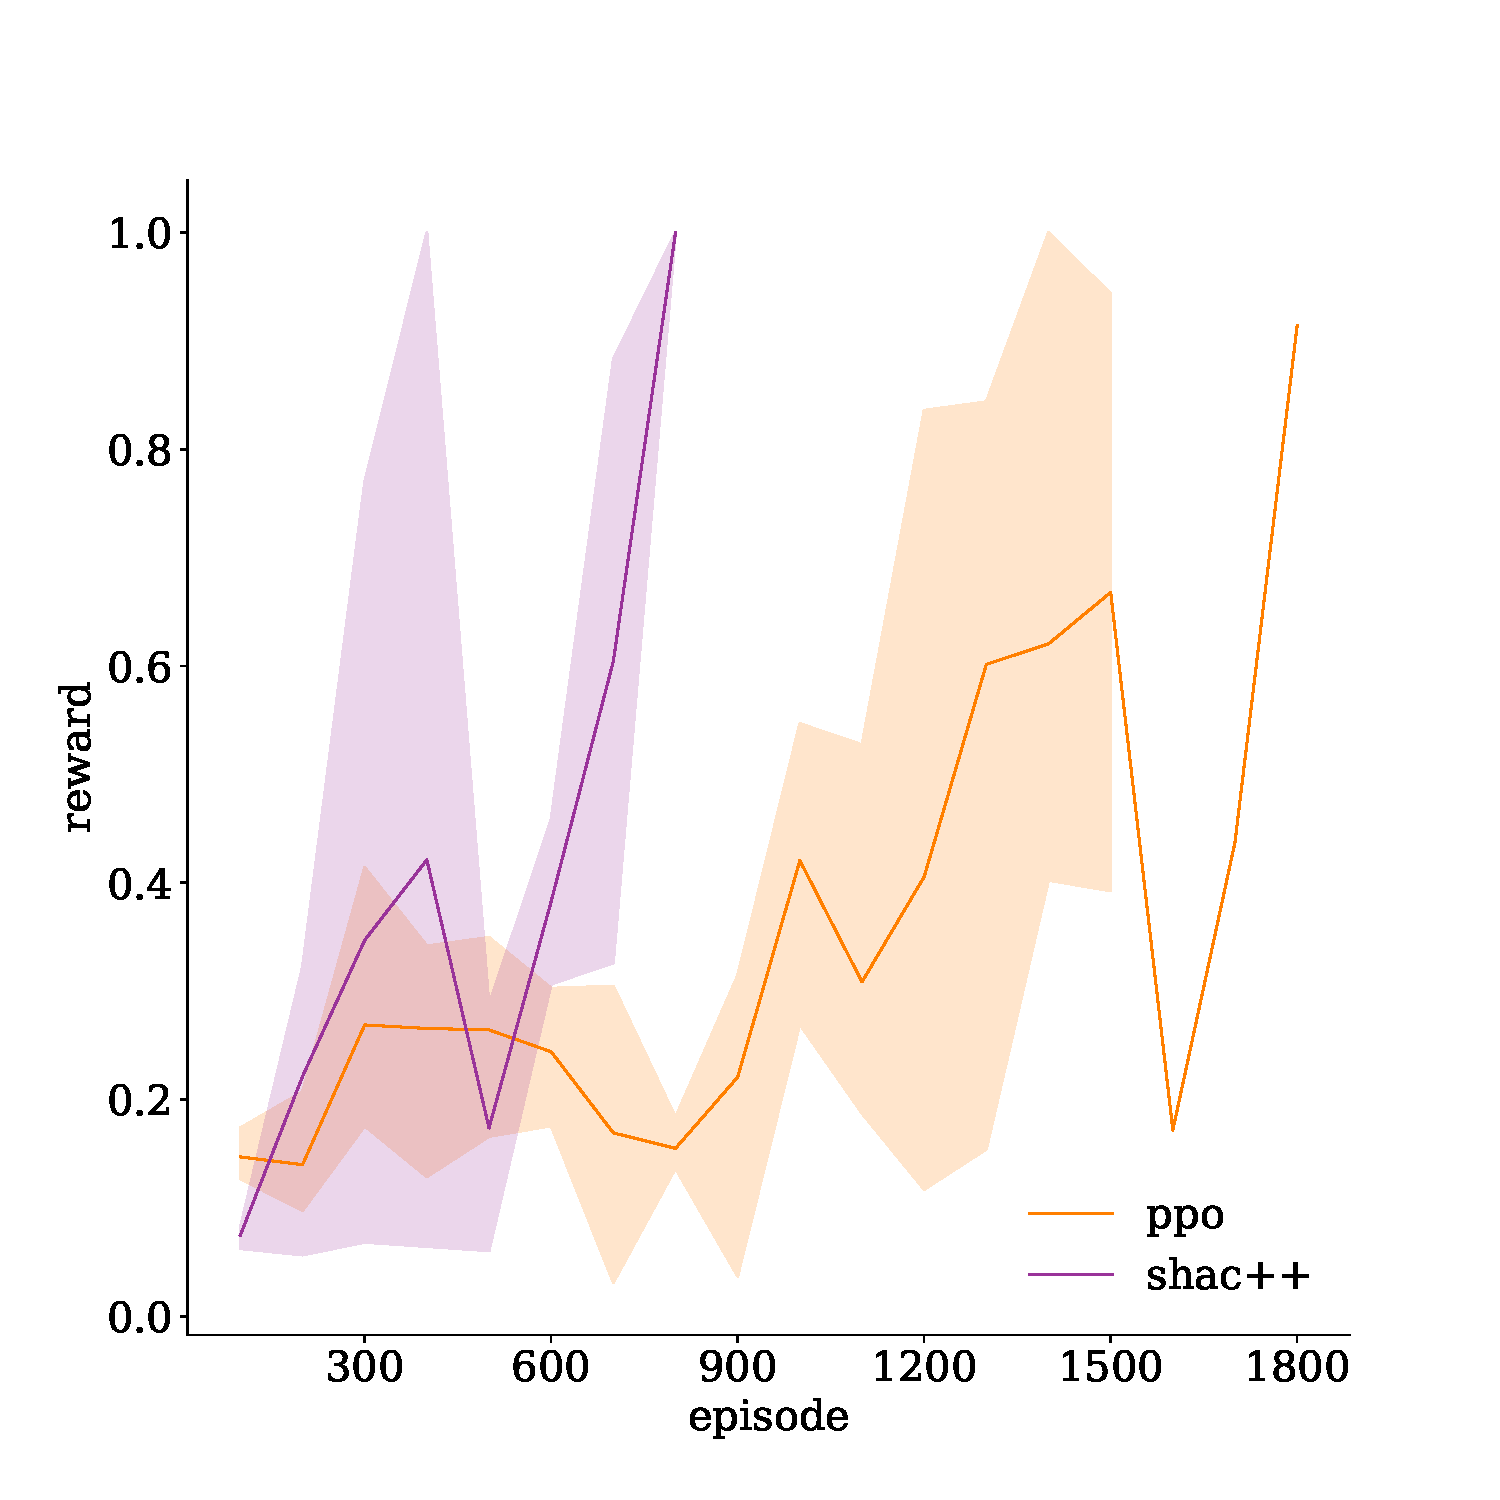
\includegraphics[width=\textwidth]{figs/dispersion-1-mlp.pdf}
        \caption{Dispersion, MLP, 1 agent}
        \label{fig:dispersion-mlp-1}
    \end{subfigure}
    \begin{subfigure}[b]{0.30\textwidth}
        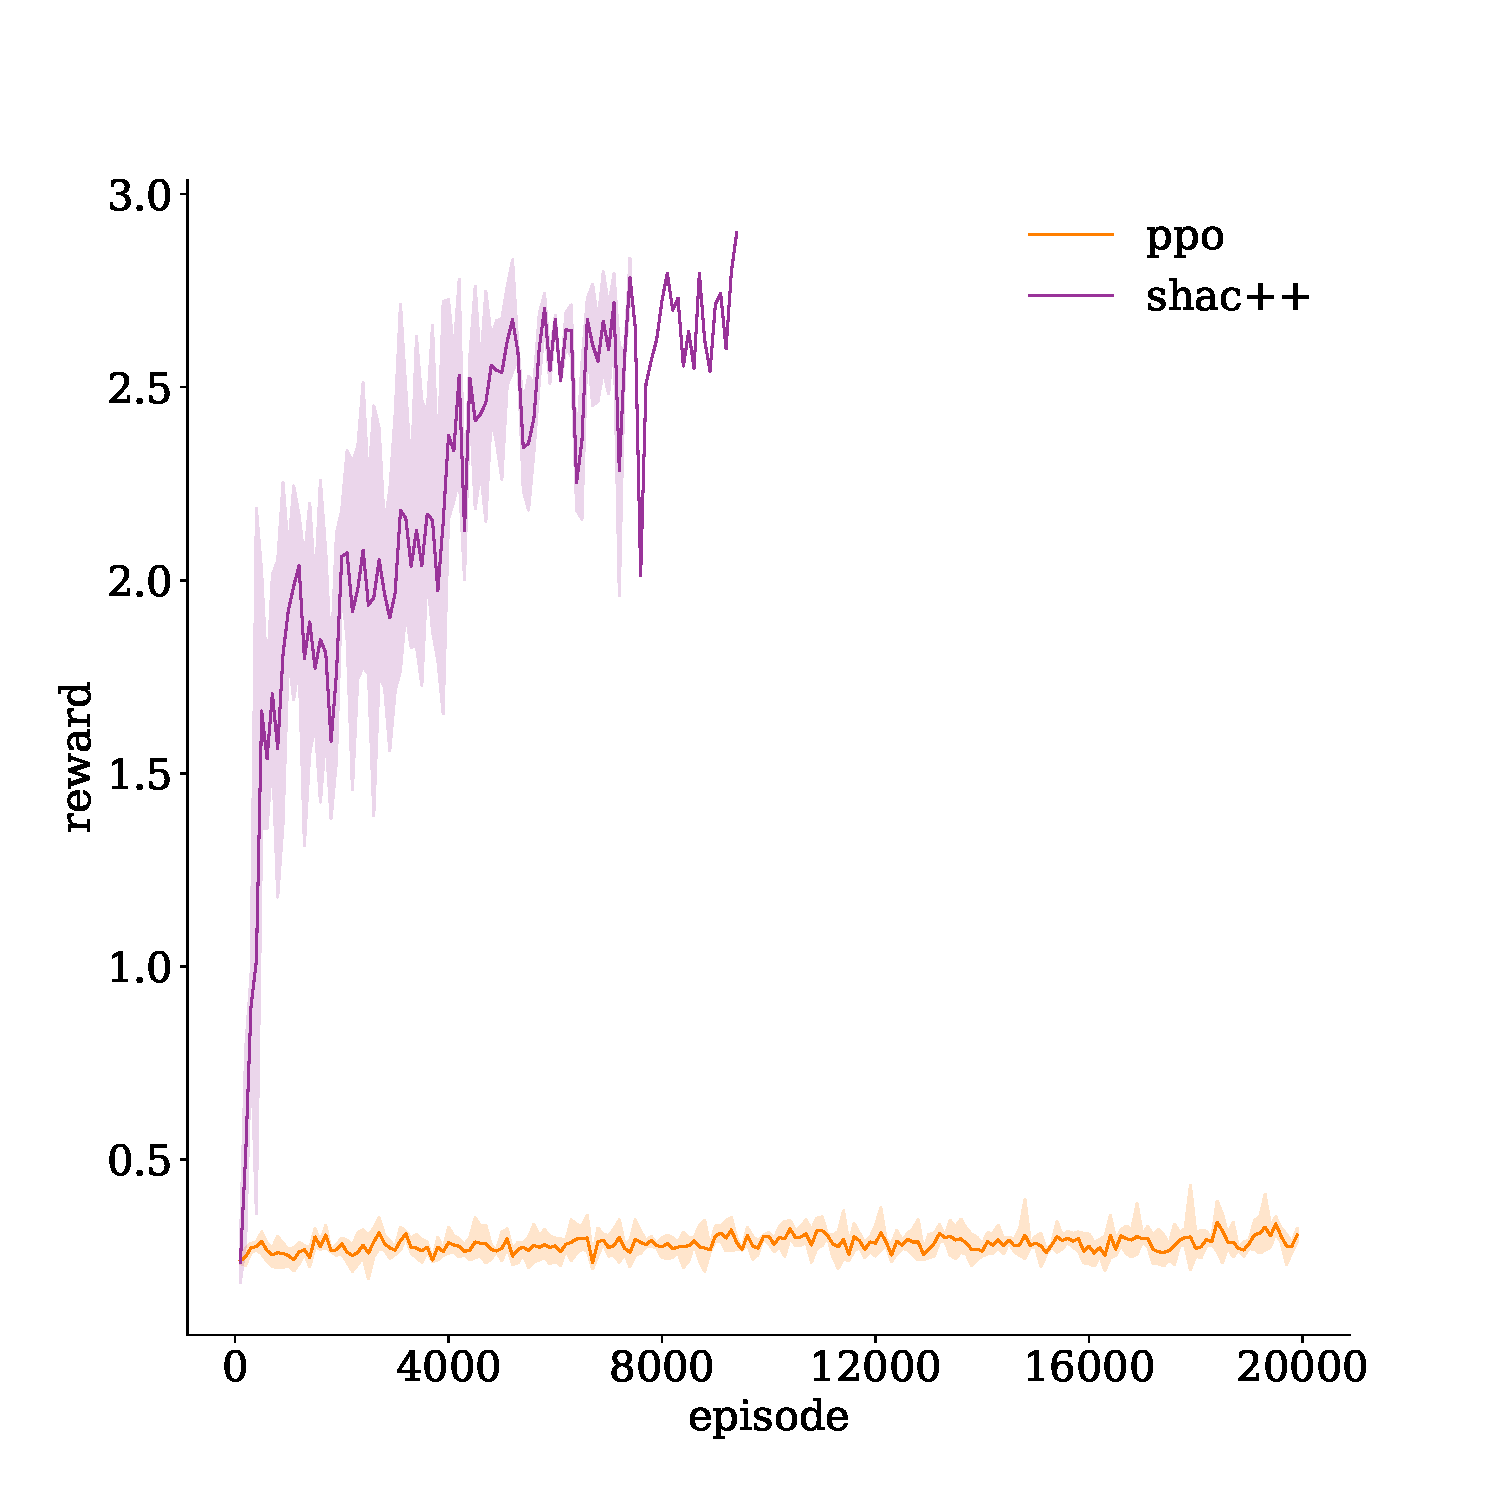
\includegraphics[width=\textwidth]{figs/dispersion-3-transformer.pdf}
        \caption{Dispersion, Transformer, 3 agents}
        \label{fig:dispersion-transformer-3}
    \end{subfigure}
    \begin{subfigure}[b]{0.30\textwidth}
        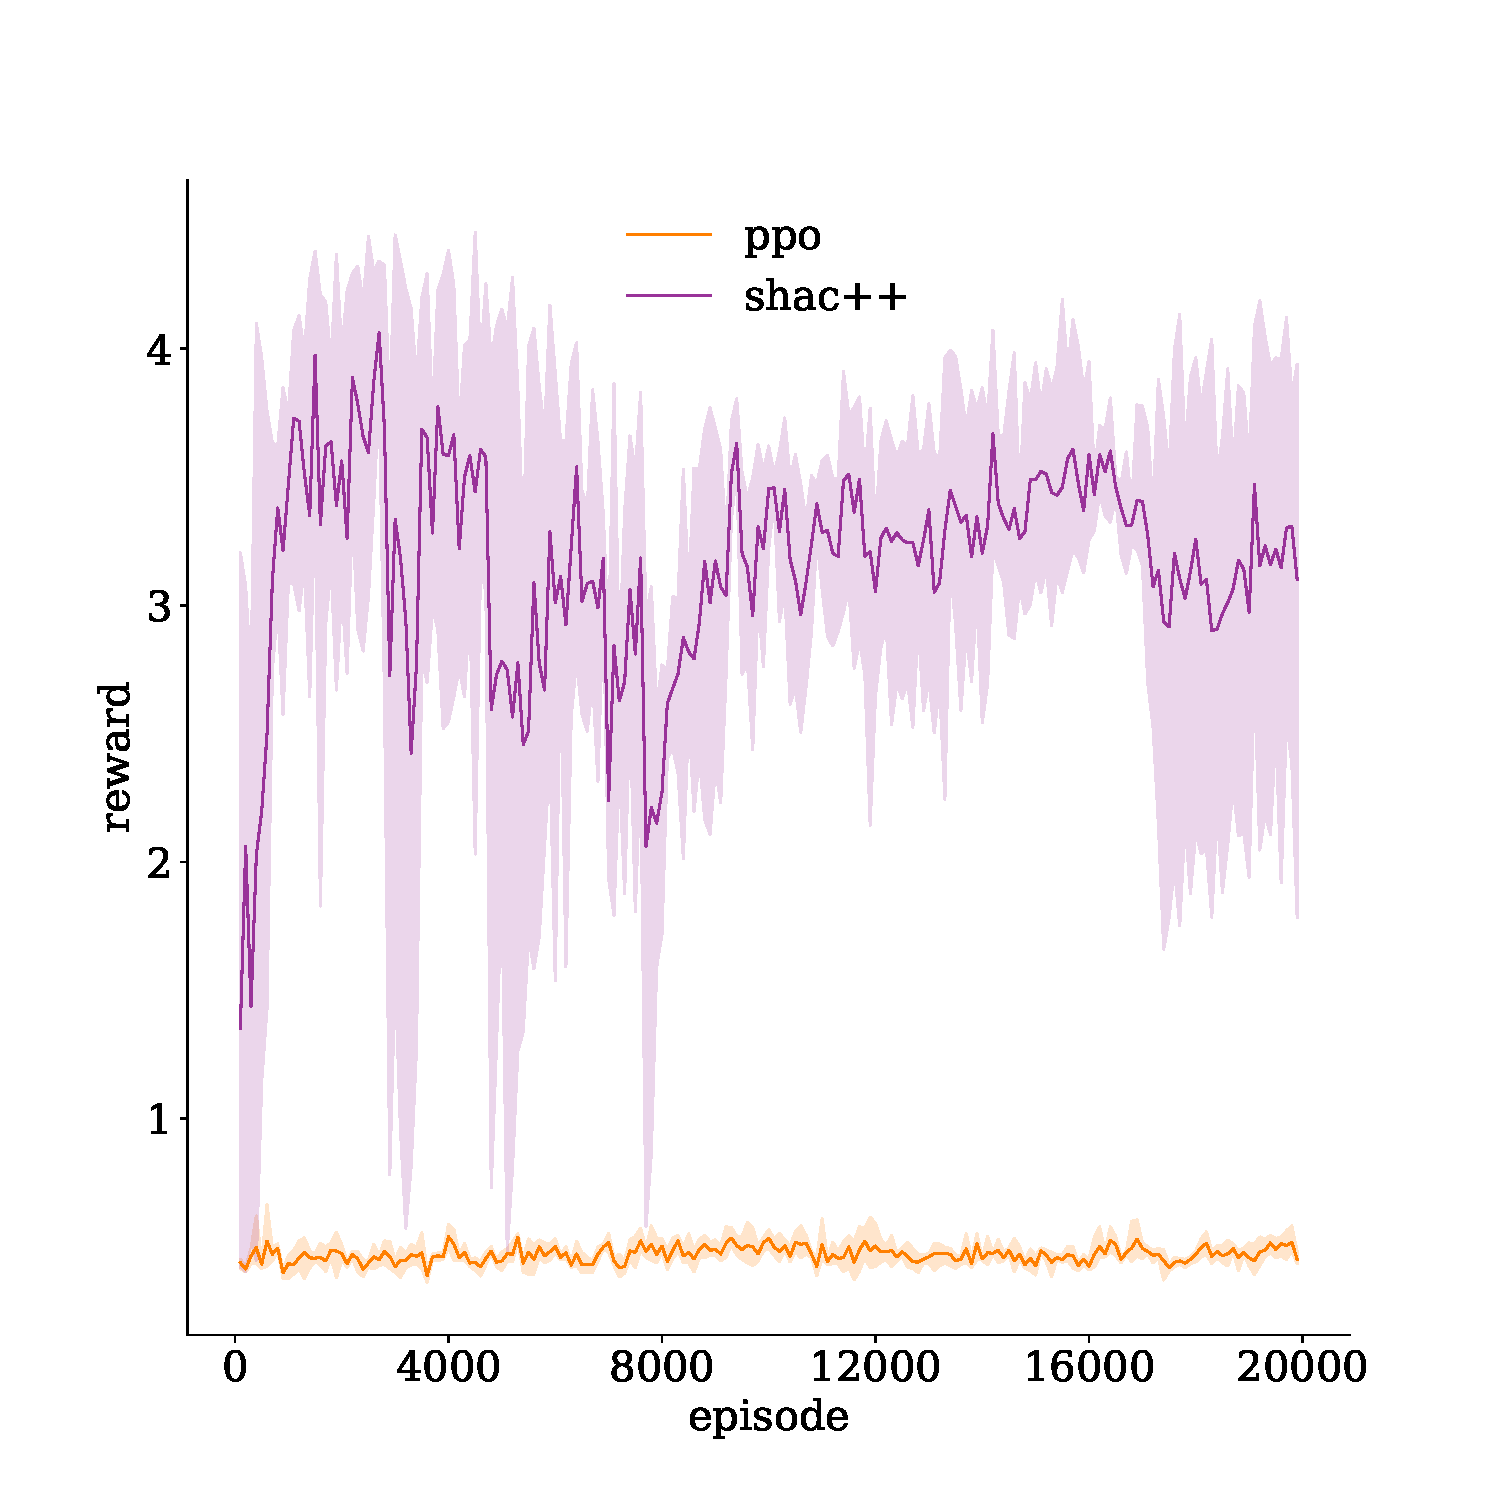
\includegraphics[width=\textwidth]{figs/dispersion-5-transformer.pdf}
        \caption{Dispersion, Transformer, 5 agents}
        \label{fig:dispersion-transformer-5}
    \end{subfigure}

    \begin{subfigure}[b]{0.30\textwidth}
        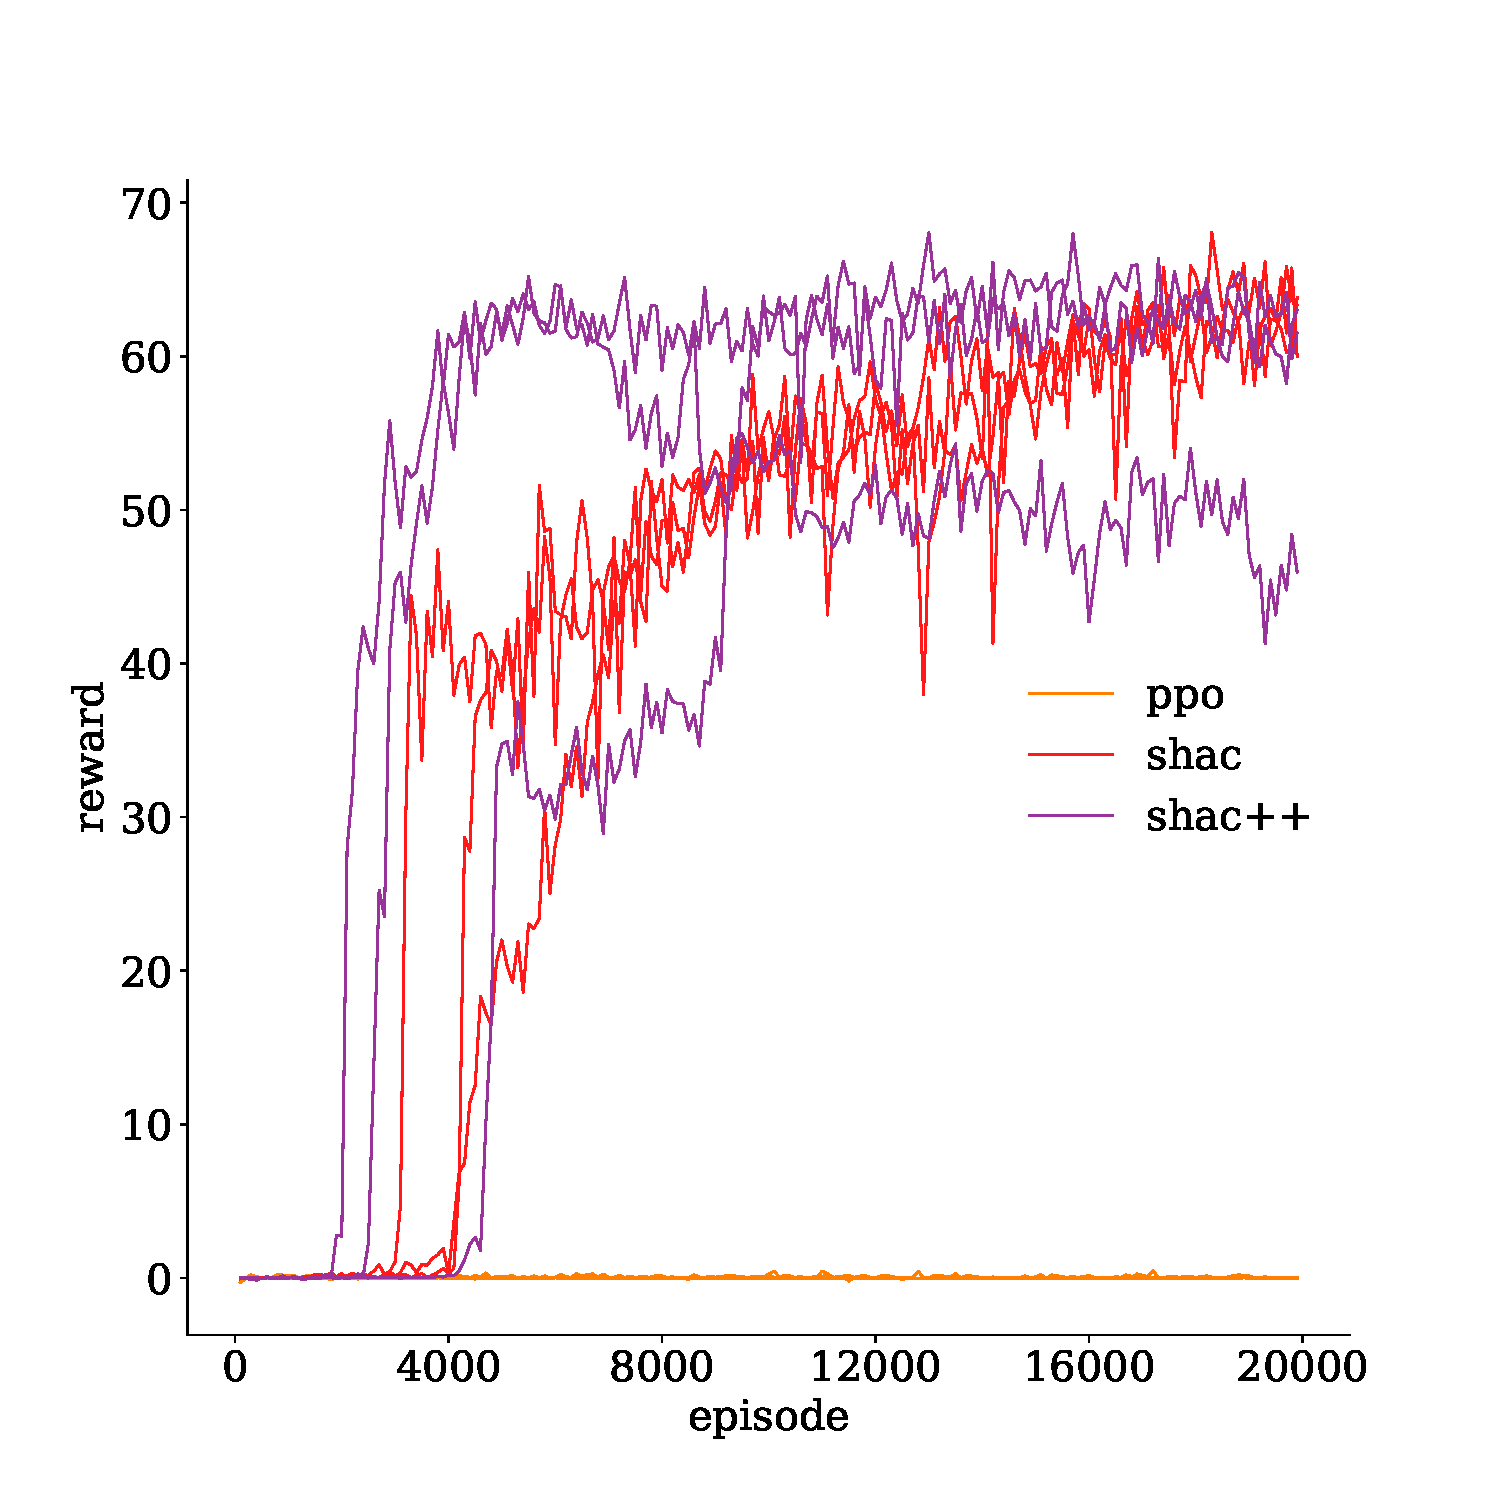
\includegraphics[width=\textwidth]{figs/transport-1-mlp.pdf}
        \caption{Transport, MLP, 1 agent}
        \label{fig:transport-mlp-1}
    \end{subfigure}
    \begin{subfigure}[b]{0.30\textwidth}
        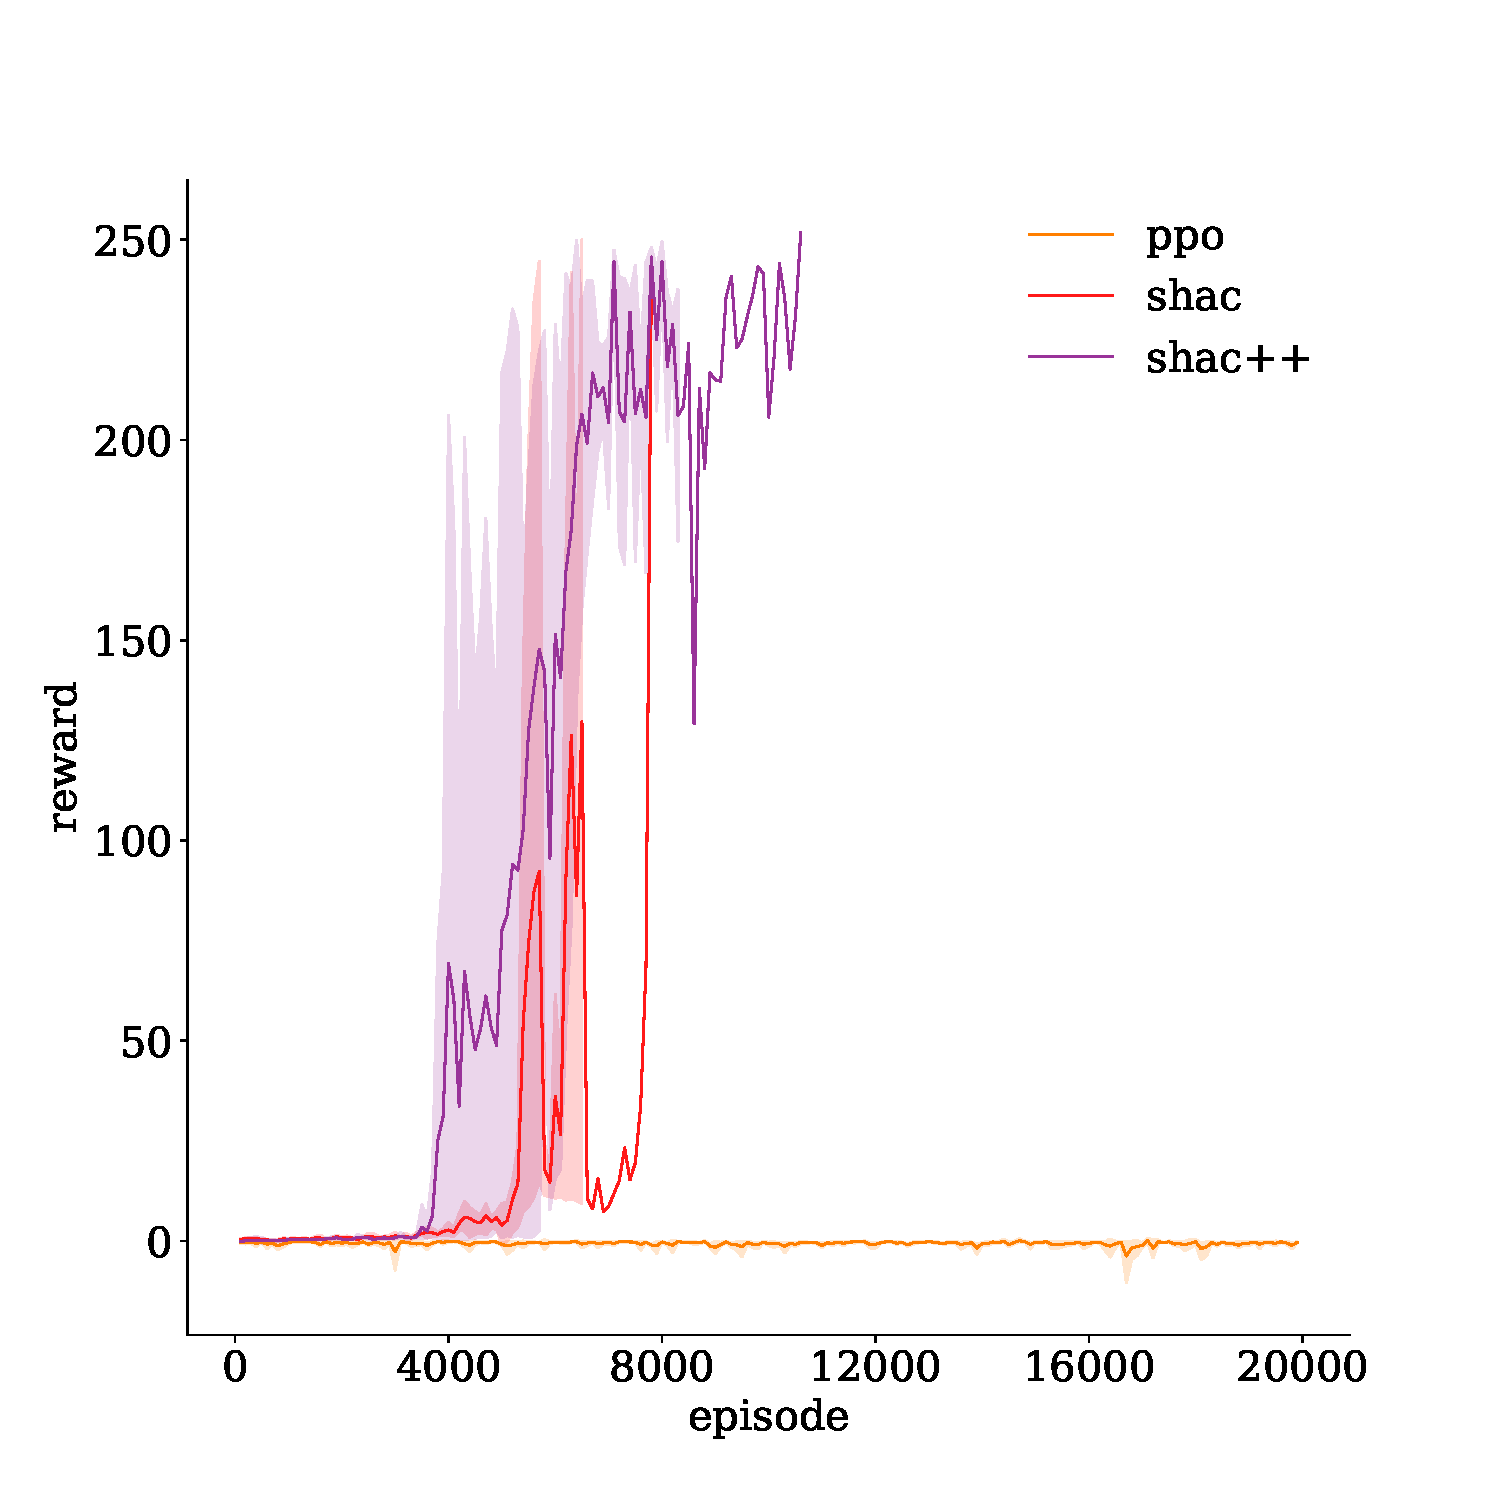
\includegraphics[width=\textwidth]{figs/transport-3-transformer.pdf}
        \caption{Transport, Transformer, 3 agents}
        \label{fig:transport-transformer-3}
    \end{subfigure}
    \begin{subfigure}[b]{0.30\textwidth}
        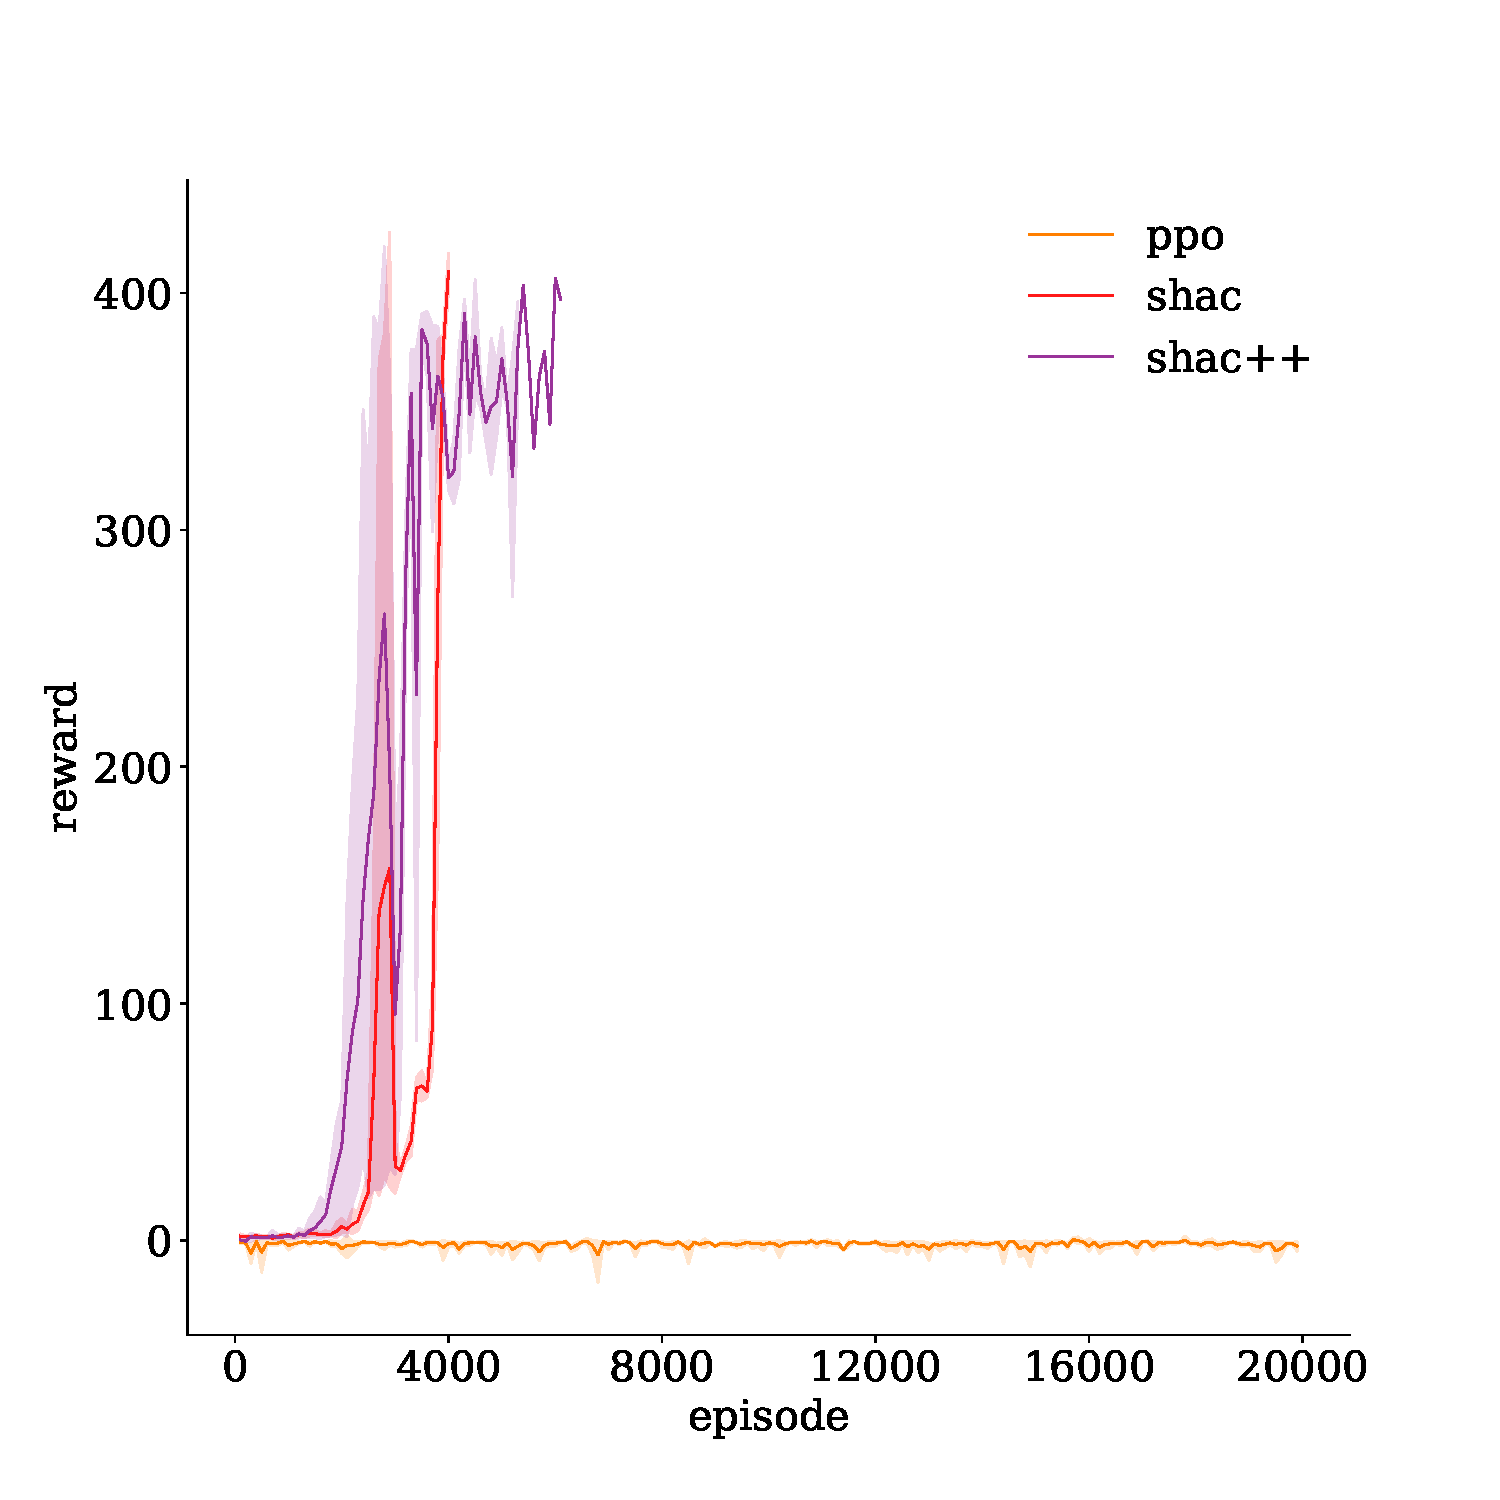
\includegraphics[width=\textwidth]{figs/transport-5-transformer.pdf}
        \caption{Transport, Transformer, 5 agents}
        \label{fig:transport-transformer-5}
    \end{subfigure}

    \begin{subfigure}[b]{0.30\textwidth}
        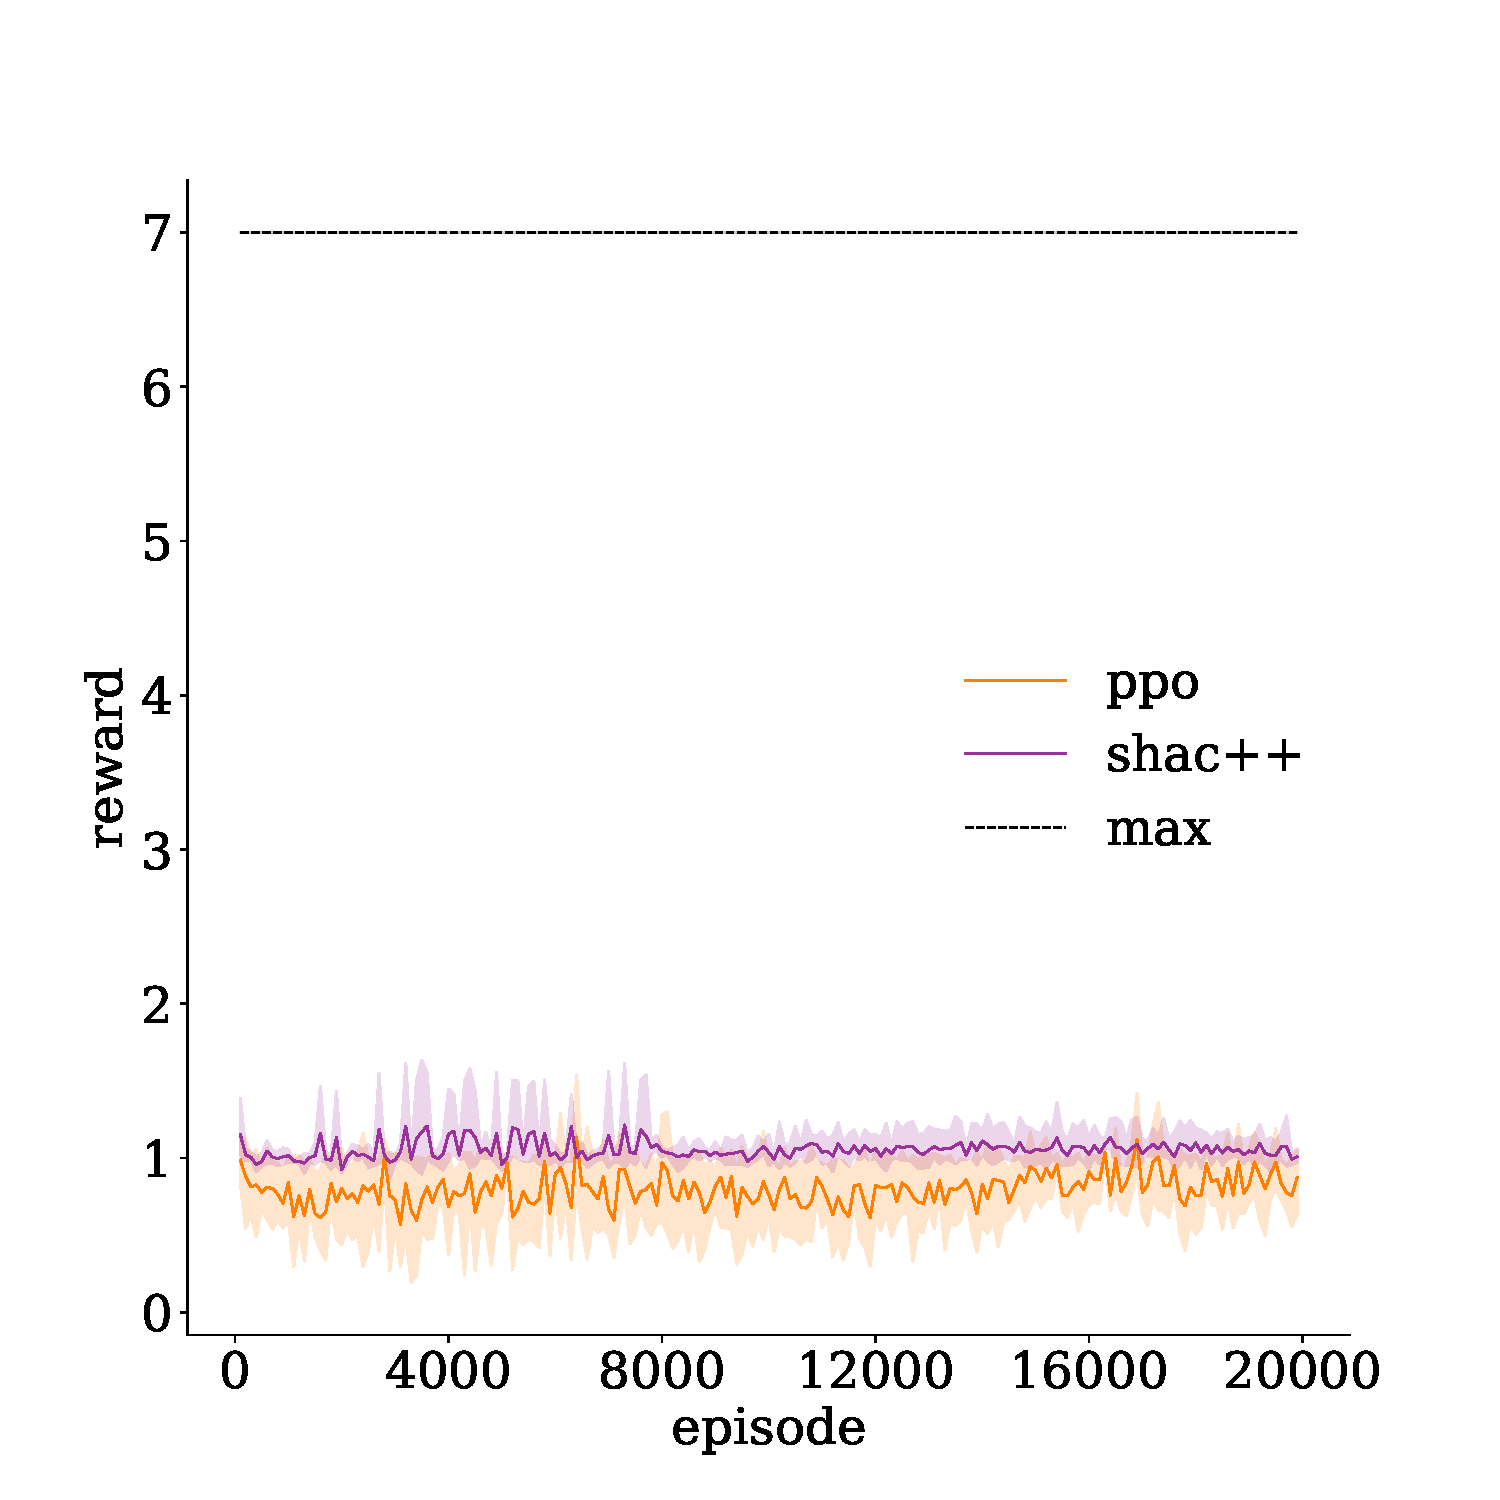
\includegraphics[width=\textwidth]{figs/discovery-1-mlp.pdf}
        \caption{Discovery, MLP, 1 agent}
        \label{fig:discovery-mlp-1}
    \end{subfigure}
    \begin{subfigure}[b]{0.30\textwidth}
        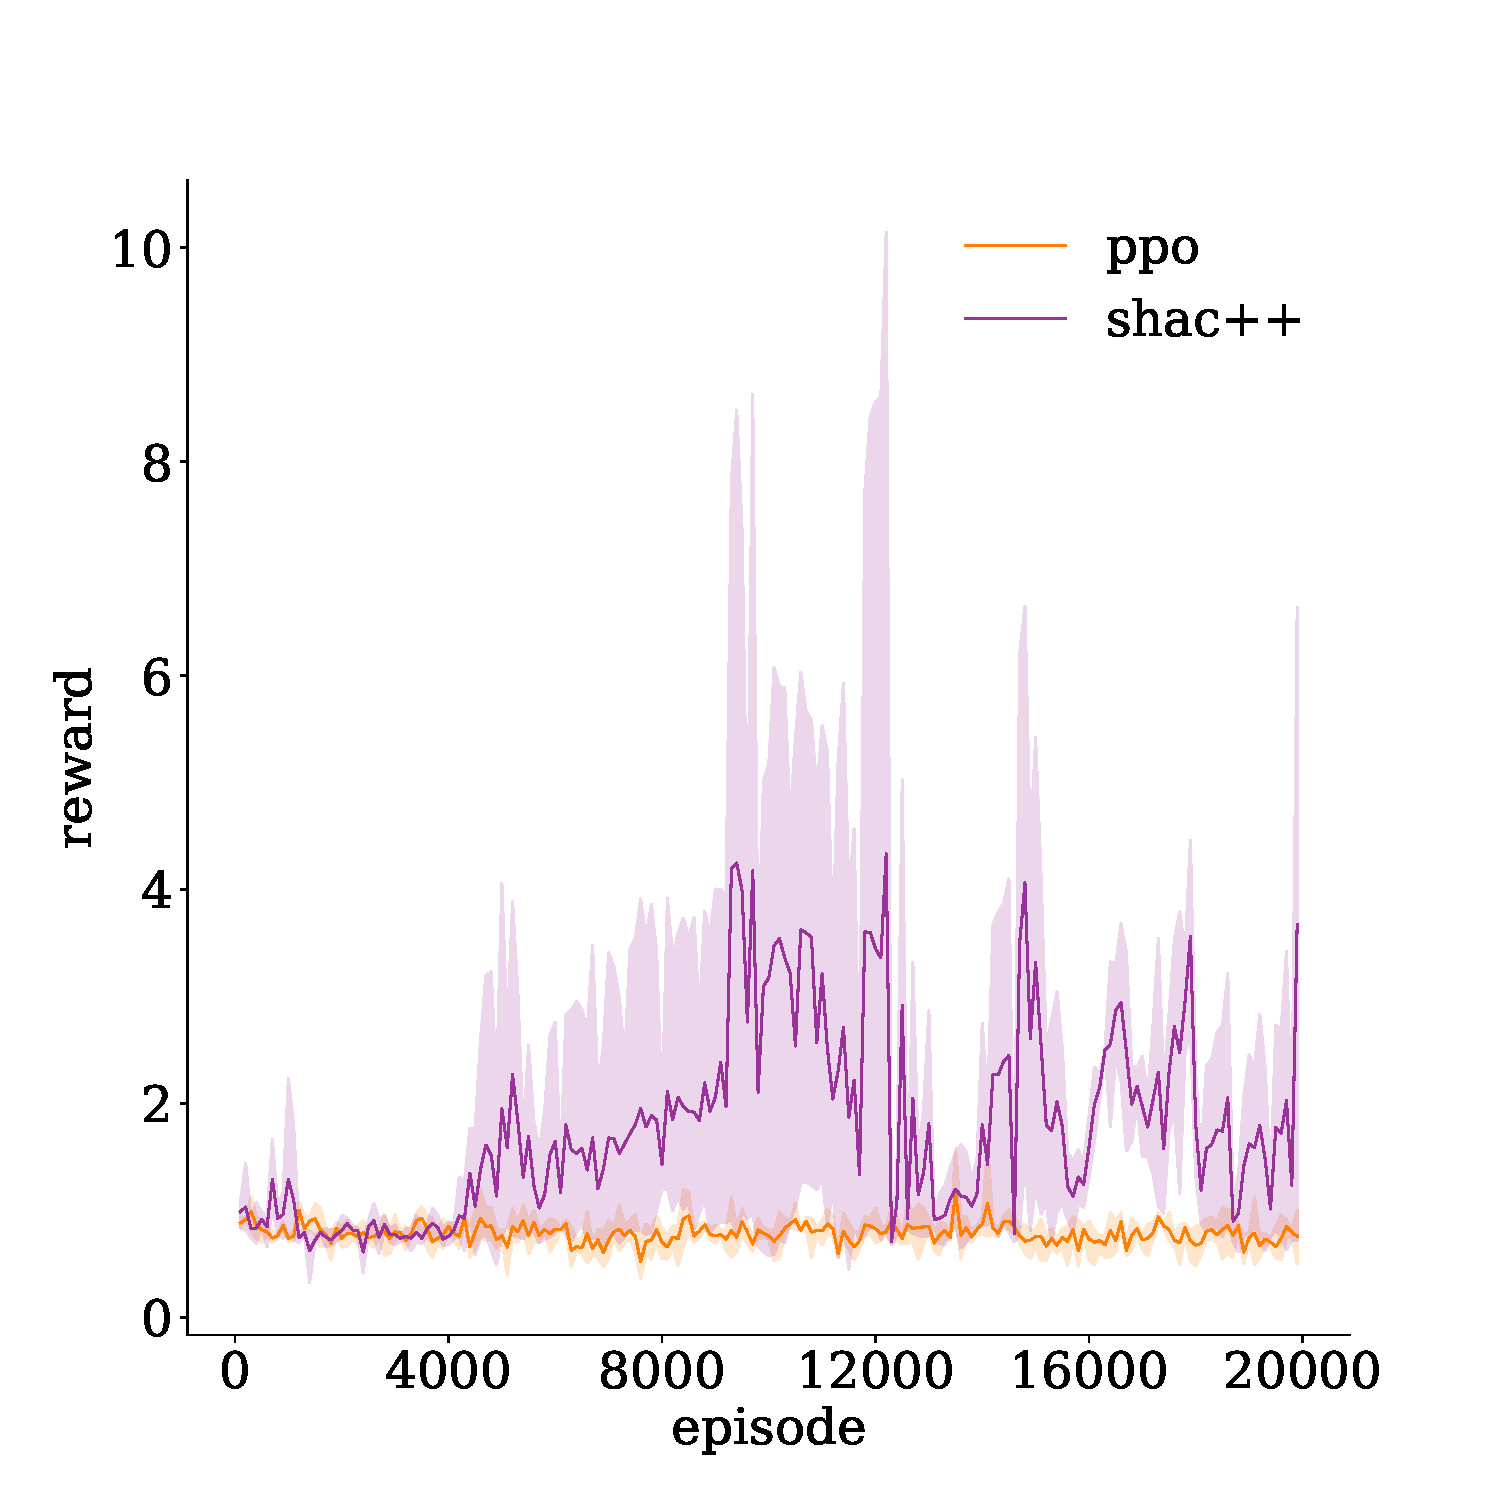
\includegraphics[width=\textwidth]{figs/discovery-3-transformer.pdf}
        \caption{Discovery, Transformer, 3 agents}
        \label{fig:discovery-transformer-3}
    \end{subfigure}
    \begin{subfigure}[b]{0.30\textwidth}
        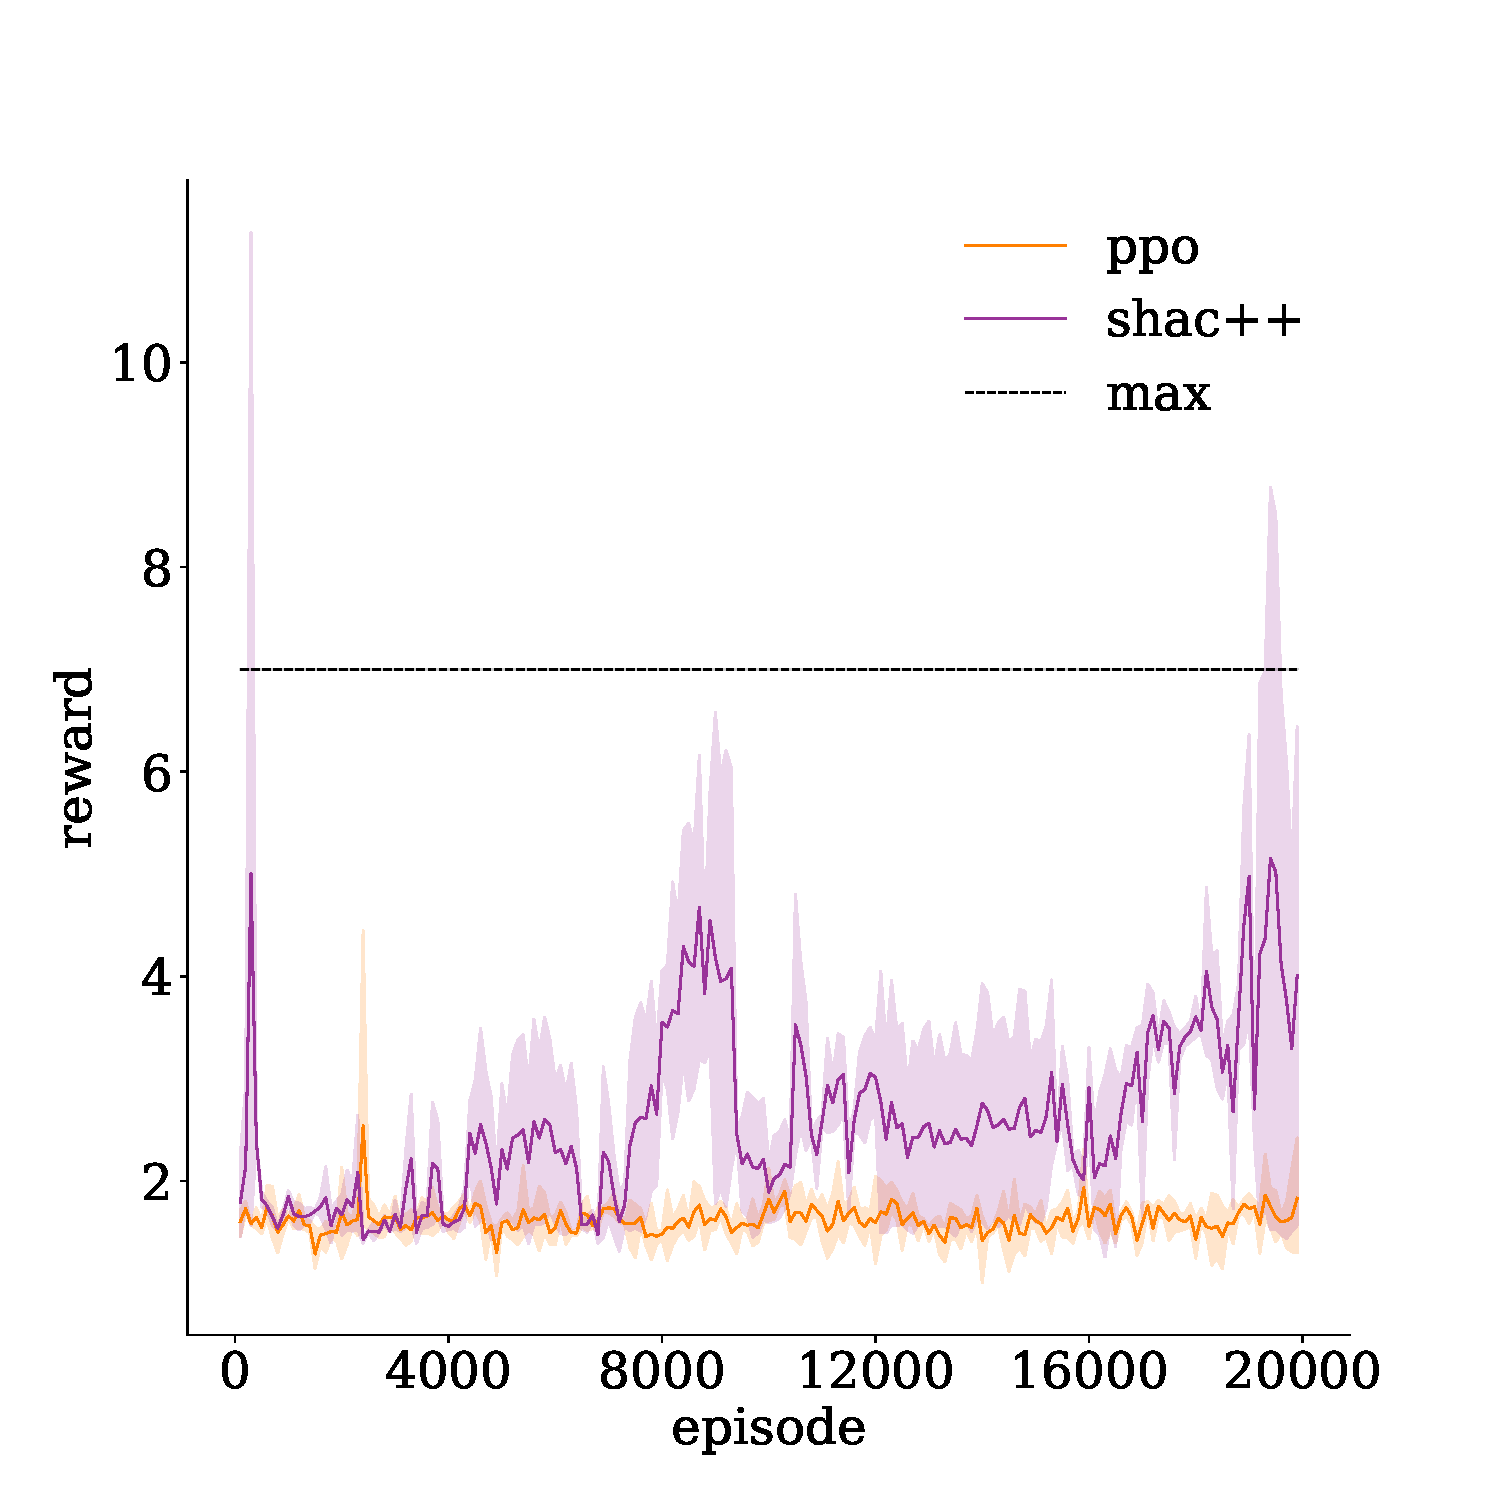
\includegraphics[width=\textwidth]{figs/discovery-5-transformer.pdf}
        \caption{Discovery, Transformer, 5 agents}
        \label{fig:discovery-transformer-5}
    \end{subfigure}

    \begin{subfigure}[b]{0.30\textwidth}
        \includegraphics[width=\textwidth]{figs/sampling-1-mlp.pdf}
        \caption{Discovery, MLP, 1 agent}
        \label{fig:sampling-mlp-1}
    \end{subfigure}
    \begin{subfigure}[b]{0.30\textwidth}
        \includegraphics[width=\textwidth]{figs/sampling-3-transformer.pdf}
        \caption{Discovery, Transformer, 3 agents}
        \label{fig:sampling-transformer-3}
    \end{subfigure}
    \begin{subfigure}[b]{0.30\textwidth}
        \includegraphics[width=\textwidth]{figs/sampling-5-transformer.pdf}
        \caption{Discovery, Transformer, 5 agents}
        \label{fig:sampling-transformer-5}
    \end{subfigure}

    \caption{Comparison between \fname{}, PPO, and SHAC for increasing number of agents for Dispersion, Transport, Discovery, and Sampling scenarios for the Transformer Architecture.}
    \label{fig:experiments}
\end{figure*}

\begin{figure}[t]
    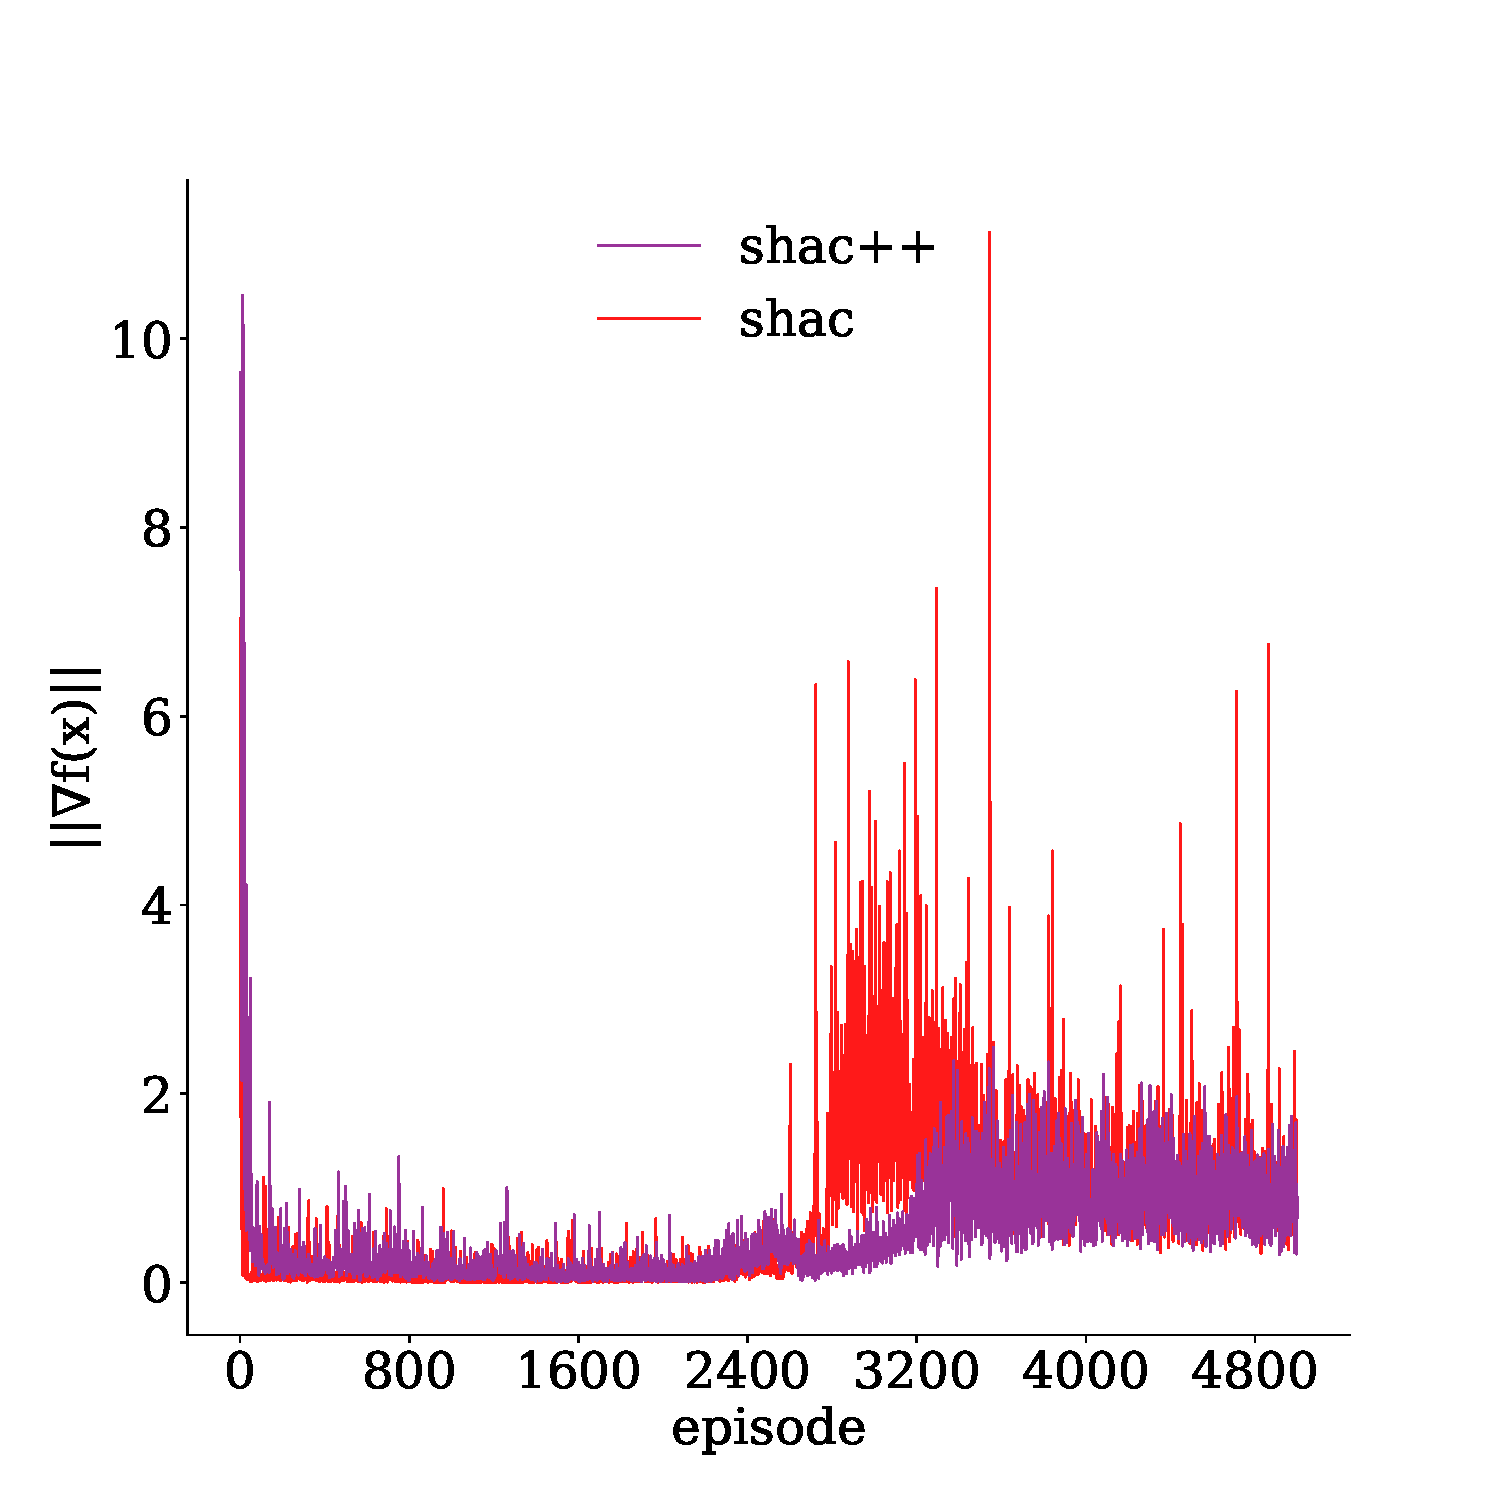
\includegraphics[width=\columnwidth]{figs/grads-transformer-transport.pdf}
    \caption{Norm of policy gradients on the Transport environment across 5000 epochs. The raise in norm for SHAC (epoch 2700) corresponds with occurence of generalization, where collision between agents and the packages become frequent. Also \fname{} experience a raise in norm, albeit more behaved, corresponds with the occurence of generalization (epoch 3200).}
\end{figure}

\section{Experiments}\label{sect:experiments}

\paragraph{Scenarios}
As mentioned previously, we choose a few multi-agent scenarios from the VMAS\footnote{\url{https://github.com/proroklab/VectorizedMultiAgentSimulator}} package to test \fname{} aganist SHAC and PPO. In particular, we choose the following scenario:
\begin{compactitem}
    \item \textbf{Dispersion} (Fig.~\ref{fig:dispersion}): 
        \sentence{Environment} a scenario where $n$ agents need to reach $n$ goal locations, in such case the agent receives a sparse reward of $1$. Agents observe only their own position, velocity and relative position to each goal. 
        \sentence{Differentiability} Despite the transition function being differentiable, the reward function is not. Therefore, only PPO and \fname{} are applicable to this scenario. 
        \sentence{World Model} The world model has enough information to predict the next states accurately.
        \sentence{Max Reward} The maximum reward is $n$.
    \item \textbf{Transport} (Fig.~\ref{fig:transport}): 
        \sentence{Environment} a scenario where $n$ agents need to collaborate to push a package into a goal location. Agents observe their own position, velocity, relative position to the package and relative position between package and the goal. The agents receive a reward proportional to the distance between package and the goal. 
        \sentence{Differentiability} In this scenario, both the reward and transition functions are differentiable. 
        \sentence{World Model} The world model has enough information to predict the next states accurately.
        \sentence{Max Reward} The maximum reward varies from environement to environment. It is the scaled distance between the package and the goal times the number of agents.
    \item \textbf{Discovery} (Fig.~\ref{fig:discovery}): 
        \sentence{Environment} a scenario where $n$ agents need to collect $k$ goal place randomly. A goal is collected if at least $s$ agents stand in proximity to it, in this case they receive a reward of $1$. If agents collide with each other, they receive a penalty. Every agent observes its position, velocity, lidar measurements to other agents and goals. When $n=1$ we set $s=1$ and $k=7$. When $n>1$ we set $s=2$.
        \sentence{Differentiability} In this scenario, only the transition function is differentiable. Therefore, only PPO and \fname{} are applicable to this scenario. 
        \sentence{Max Reward} The maximum rewards depends on the number evaluation steps, but for early stopping purposes, we set it to $k$. 
        \sentence{World Model} Note that, a world model (or an action world model) that uses only the agents observation cannot predict the evolution correctly, as goals may not be visible to the agents. For this reason, this scenario is particularly challenging for \fname{} as we do not provide the full world state to the world model.
     \item \textbf{Sampling} (Fig.~\ref{fig:sampling}): 
        \sentence{Environment} a scenario where $n$ agents need to collect rewards from a grid. The reward are sampled from $k$ gaussians. Agents observe their own position, velocity, lidar values to each other, and rewards in a 3x3 grid around themselves.  
        \sentence{Differentiability} In this scenario, both the reward and transition functions are differentiable. 
        \sentence{Max Reward} The maximum reward depends on where the gaussians are placed.
        \sentence{World Model} Similarly to discovery, this scenario is particularly challenging for \fname{} as we do not provide the full world state, but only the agents observations, to the world model.
\end{compactitem}

\begin{table*}[!t]
    \centering
    \input tables/max.tex
    \caption{Normalized maximum rewards (relative to the best performing model) for the different scenarios.}
\end{table*}

\paragraph{Architectures}
We test SHAC, PPO, and \fname{} with both an MLP and a Transformer architecture. Specifically, we use a 1-layer MLP with hidden size 64 or a 1-layer single-head Transformer with hidden size 64 for the Policy Network and Value Network (for PPO, SHAC, and \fname{}). For the Reward Network, we use a 1-layer MLP with hidden size 64 or a 1-layer single-head Transformer with hidden size 64 (for \fname{}). The Transition Network for \fname{} is a 3-layer single-head Transformer with hidden size 64.

While the MLP architecture is the simplest, the Transformer baseline benefits from position invariance property of the agents observations. We apply the transformer architecture only if the number of agents is greater than $1$, otherwise we use only the MLP architecture. 

\paragraph{Hyperparameters}
For all networks we use learning rate of $1e\text{-}3$ with Adam Optimizer~\cite{Kingma14}. For all scenarios, each training episode consists of $512$ environments of $32$ steps each. Each validation episode is composed of $512$ environments of $512$ steps each. We employ early stopping when the agents achieve $90\%$ of the maximum reward in $90\%$ of the episode's environments. If early stopping is not triggered, we stop training after $20,000$ episodes. The discount factor is set to $0.99$ and lambda factor is set to $0.95$. We report results for increasing number of agents $n\in\{1,3,5\}$. We repeat and report results for $3$ runs with different seeds. See Table~\ref{apx:tab:ppo} and Table~\ref{apx:tab:shac} for a complete list of hyperparameters.

Overall, considering different training algorithms, architectures, scenarios, hyperparameters, we completed a total of $254$ runs lasting between $1$ to $8$ hours each. 

\paragraph{Hardware Setup}
Our experiments were conducted on a cluster of machines composed of 2 computational nodes, each with one Nvidia Tesla V100 GPU (with 32GB of memory), 200GB of RAM, and two Intel Xeon Gold 6226R processors (32 cores each).

\subsection{Results}

\paragraph{Dispersion}
Firstly, we compare the performance of these algorithms on a non-differentiable scenario (thus SHAC is not aplicable), dispersion. We show the comparison between \fname{} and PPO for increasing number of agents for the transformer architecture (see Fig.~\ref{apx:fig:experiments-mlp}). In single agent setting, show in Fig.~\ref{fig:dispersion-mlp-1}, both algorithm perform well, albeit \fname{} tends to converge after fewer episodes. With $3$ agents, shown in Fig.~\ref{fig:dispersion-transformer-3}, PPO fails to converge, meanwhile \fname{} converges in less than $10,000$ episodes. With $5$ agents, shown in Fig.~\ref{fig:dispersion-transformer-5}, PPO fails to converge, meanwhile \fname{} achieves high rewards without however triggering the early stopping. In this last scenario, \fname{} manifest also high reward variance.

\paragraph{Transport}
Now, we compare the performance of these algorithms on a fully differentiable scenario, transport. On the single agent setting, shown in Fig.~\ref{fig:transport-mlp-1}, PPO fails to converge, meanwhile both SHAC and \fname{} perform similarly well. While \fname{} appears to converge earlier SHAC appear to be more consistent. With $3$ and $5$ agents, shown in Fig.~\ref{fig:transport-transformer-3} and \ref{fig:transport-transformer-5}, PPO fails to converge, meanwhile both SHAC and \fname{} perform similarly well albeit SHAC is more stable. For the MLP only setting see Fig.~\ref{apx:fig:experiments-mlp} 

\paragraph{Discovery}
Similar consideration hold also for the discovery scenario. In the single agent setting, shown in Fig.~\ref{fig:discovery-mlp-1}, \fname{} performs better, but comparitavely, to PPO . However, with $3$ and $5$ agents, shown in Fig.~\ref{fig:discovery-transformer-3} and \ref{fig:discovery-transformer-5}, PPO fails to converge, meanwhile \fname{} performs better. For the MLP only setting see Fig.~\ref{apx:fig:experiments-mlp} 

\paragraph{Sampling}


